\documentclass[pdflatex,sn-mathphys-num]{sn-jnl}

\usepackage{graphicx}
\usepackage{multirow}
\usepackage{amsmath,amssymb}
\usepackage{booktabs}
\usepackage{array}
\usepackage{tabularx}
\usepackage{enumitem}
\usepackage{xcolor}
\usepackage{tikz}
\usepackage{pgfplots}
\usepackage{hyperref}
\hypersetup{hypertexnames=false}
\usepackage{url}
\usepackage{placeins}
\usetikzlibrary{arrows.meta,positioning,shapes.geometric,fit,calc}
\pgfplotsset{compat=1.18}

\tikzset{
  paperbox/.style={draw=blue!60!black, fill=blue!8, rounded corners, minimum width=3.3cm, text width=3.3cm, minimum height=0.85cm, align=center, font=\small},
  papersmall/.style={draw=teal!70!black, fill=teal!10, rounded corners, minimum width=2.7cm, text width=2.7cm, minimum height=0.75cm, align=center, font=\small},
  paperdecision/.style={diamond, draw=orange!80!black, fill=orange!12, aspect=2.0, text width=2.8cm, inner sep=1.2pt, align=center, font=\small},
  paperarrow/.style={-Latex, thick}
}

\title[Confidence-Calibrated LLM Code Review]{Confidence-Calibrated LLM with Selective Abstention for Reliable Automated Code-Review Triage: A Hybrid Pipeline Combining Post-Hoc Calibration, Conformal Gating, and Rule Corroboration}

\author*[1]{\fnm{Rehan}}
\affil*[1]{\orgname{Lovely Professional University}, \country{India}}

\abstract{Large language models (LLMs) can assist vulnerability review, but a model that flags nearly every function creates a large false-positive burden. This paper evaluates a selective code-review pipeline that calibrates an open-source code LLM, abstains on uncertain decisions, and uses Semgrep as independent rule-based corroboration. We audit the raw PrimeVul v0.1 train, validation, and test partitions before evaluation, using memory-bounded approximate similarity retrieval followed by token-overlap verification and provenance review. The final leakage-controlled validation and test populations contain 23,033 and 24,008 records, respectively. Qwen2.5-Coder-1.5B-Instruct is evaluated with a code-only prompt. On the locked test partition, raw Qwen produces positive alerts for 99.08\% of records, with 2.01\% precision among alerts and 91.76\% vulnerable-record recall. The frozen calibrated and Semgrep-corroborated policy accepts 1.88\% of records, increasing accepted-alert precision to 7.96\% while reducing vulnerable-record recall to 6.90\%. The precision improvement over raw Qwen is +5.95 percentage points under both record-level and project-clustered sensitivity analyses. A separate 400-project candidate evaluation shows the operating-point trade-off: increasing the conformal level from 0.10 to 0.50 raises coverage from 2.89\% to 8.01\% and recall from 11.32\% to 25.23\%, but decreases precision from 11.01\% to 8.86\%. The results support selective review triage rather than fully autonomous vulnerability detection.}

\keywords{large language models, vulnerability detection, automated code review, confidence calibration, selective prediction, conformal prediction, static analysis, Semgrep, PrimeVul}

\begin{document}
\maketitle

\section{Introduction}\label{sec:introduction}

Large language models have become useful assistants for programming, code understanding, testing, and software maintenance. Recent literature includes surveys of automated code review and software-quality evaluation, empirical studies of LLM vulnerability detection, and hybrid systems that combine LLM reasoning with static analysis \cite{Borgalli2026,TaghaviFar2025,Tamberg202529698,Gnieciak2025198410}. However, capability is not the same as dependable deployment. In a security-review workflow, an incorrect positive alert consumes developer attention, while an incorrect negative decision can leave a vulnerability unreported.

This problem is especially visible when an LLM is used as a binary code classifier. A model may appear to have high recall because it flags almost every record, while the resulting alert stream is too noisy for practical use. The system therefore needs a way to distinguish predictions that can be accepted automatically from cases that should be escalated to a human reviewer.

This paper implements and evaluates a pipeline with three controls. First, post-hoc calibration adjusts the interpretation of model confidence using validation data. Second, selective prediction allows the system to abstain when the available evidence is insufficient. Third, rule corroboration uses Semgrep to provide an independent code-pattern signal. The purpose is not to remove human review, but to create a more useful high-confidence triage mode.

The study makes the following contributions:
\begin{enumerate}[leftmargin=*]
\item It provides a leakage-aware audit of the raw PrimeVul v0.1 partitions, including approximate near-duplicate retrieval, lexical verification, and provenance review.
\item It evaluates an open-source code LLM under a deterministic, code-only prompt and reports raw, calibrated/selective, static-only, and hybrid comparisons.
\item It quantifies the precision--coverage--recall trade-off of selective review on an official locked test partition.
\item It reports record-level and project-clustered bootstrap intervals and separately evaluates a project-held-out candidate without retuning the locked test.
\end{enumerate}

The main result is deliberately limited: the frozen hybrid improves precision among accepted alerts, but it does not improve every metric simultaneously and should not be described as a high-recall autonomous detector.

\section{Literature Review}\label{sec:literature}

\subsection{Search strategy and thematic organization}

The literature search was conducted in Scopus using title, abstract, and keyword fields. The export supplied for this study contains 77 records, exported on 28 October 2026. The records were organized into four themes: (i) LLMs for code review and vulnerability detection, (ii) static analysis and hybrid verification, (iii) reliability, explainability, and risk-aware deployment, and (iv) benchmark and evaluation practice. The directly relevant records are cited below; the complete export and BibTeX file are retained as research artifacts.

The search was intentionally broad. Requiring an article to mention LLMs, vulnerability detection, calibration, conformal prediction, and static analysis simultaneously would omit papers that inform only one part of the research design. The review therefore combines thematic searches and uses the methods literature to connect the themes.

\subsection{LLMs for automated code review and vulnerability detection}

Recent surveys position LLMs and automated machine learning as complementary approaches to code review, defect prediction, software quality assessment, and vulnerability detection, while identifying reliability, human verification, and cross-project generalization as unresolved issues \cite{Borgalli2026,Jelodar2026}. Domain-specific studies include SecureQwen for Python vulnerability detection, vulnerability-specific fine-tuning, and empirical evaluation of LLMs at project scale \cite{Mechri2025,Li2026}. Benchmarking studies show that results depend strongly on the dataset, prompting strategy, model family, and evaluation prevalence \cite{Tamberg202529698,Gnieciak2025198410}.

The recent Scopus literature also includes models that enrich LLMs with program structure. Examples include code-semantic transformers, graph representations, risk-path extraction, and structured knowledge for vulnerability detection \cite{Wei20262204,Dong20261,Feng2026,Liao202636005}. These approaches aim to improve the representation of code or the reasoning context, but they generally emphasize detection quality rather than the reliability of the confidence attached to each decision.

\subsection{Static analysis and hybrid LLM systems}

Static analysis is attractive because its rules are explicit and auditable, but warnings often require manual validation. Recent work uses LLMs to inspect or resolve static-analysis warnings, combines chain-of-thought reasoning with code analysis, and integrates SAST with LLM-generated code enhancement or security patching \cite{Wen2024,Huang2026,Lee2026,Alrashedy2025}. Other studies explicitly integrate LLMs and static analysis for source-code vulnerability detection \cite{Ciavatta2026}. Warning-validation work such as SNIPTEST further emphasizes that producing a warning and confirming that a warning corresponds to an exploitable issue are different tasks \cite{Murali2026}.

The literature therefore supports a complementary design: static analysis can provide interpretable pattern evidence, while an LLM can provide broader semantic reasoning. However, agreement between two tools should not automatically be interpreted as proof of correctness. Their errors may be correlated, and the absence of a static finding is not proof that code is safe. The present study treats Semgrep as corroborating evidence and measures its contribution through ablation rather than assuming independence.

\subsection{Reliability, calibration, and selective prediction}

Confidence calibration asks whether a model's confidence corresponds to its observed correctness. Temperature scaling provides a simple post-processing calibration method, while Platt scaling maps raw scores through a learned sigmoid \cite{Guo2017Calibration,Platt1999Probabilistic}. Selective classification, also called classification with a reject option, formalizes the ability to refuse uncertain cases and studies the resulting risk--coverage trade-off \cite{Geifman2017Selective}. Conformal prediction provides prediction sets or thresholds with distribution-free, finite-sample validity under its assumptions and is a natural foundation for calibrated escalation \cite{Angelopoulos2023Conformal}.

Within the retrieved software-engineering literature, calibration and risk-aware acceptance appear less developed than model construction and point-estimate detection. Risk-aware verification and explainability studies are beginning to address this gap by combining model outputs with structured checks, explanations, or model checking \cite{Alharby2026,Dubey2026,Ahmad20253321}. The present work focuses on a concrete operational form of this idea: an accepted positive alert must pass a validation-derived conformal gate and receive at least one Semgrep finding.

\subsection{Benchmarks, provenance, and the research gap}

PrimeVul is particularly relevant because its creators document label-quality, duplication, and evaluation concerns in code-language-model vulnerability detection \cite{Ding2024PrimeVul}. The supplied data include project, commit, function, and vulnerability metadata, making it possible to audit cross-partition relationships before testing. This matters because a near-duplicate or related historical version in both development and evaluation can create an overly optimistic generalization estimate.

The literature motivates the present study but does not determine its result. Existing work demonstrates strong code reasoning, static-analysis integration, and vulnerability-specific modeling, while the remaining gap is operational reliability under natural benchmark prevalence: when should the system accept an alert, when should it abstain, and how much coverage is lost in exchange for higher precision? This paper addresses that gap with a reproducible selective-review experiment rather than claiming universal superiority over prior models.

\section{Research Questions}\label{sec:rqs}

The empirical study addresses the following questions:
\begin{enumerate}[leftmargin=*]
\item \textbf{RQ1:} How does the raw open-source LLM compare with calibrated/selective, static-only, and hybrid decisions on precision, coverage, and vulnerable-record recall?
\item \textbf{RQ2:} Does validation-only post-hoc calibration provide a usable confidence signal for selective acceptance?
\item \textbf{RQ3:} Does conformal-style abstention improve precision among accepted alerts, and what is the coverage cost?
\item \textbf{RQ4:} Does Semgrep corroboration improve accepted-alert precision when used as an intersection gate?
\item \textbf{RQ5:} Does the precision--coverage--recall trade-off persist on a separate project-held-out candidate without changing the official locked-test result?
\end{enumerate}

\section{Methods}\label{sec:methods}

\subsection{Dataset and ground truth}

The primary dataset is PrimeVul v0.1. The task is function-level binary vulnerability classification: target 1 denotes a vulnerable function and target 0 denotes a non-vulnerable function. The raw partitions contain 175,797 training records, 23,948 validation records, and 24,788 test records, for 224,533 records in total. The raw JSONL files were not modified.

\begin{table}[htbp]
\caption{Raw PrimeVul partitions and leakage-controlled evaluation roles.}\label{tab:dataset}
\centering
\begin{tabular}{@{}lrrrr@{}}
\toprule
Partition & Raw records & Target 1 & Excluded & Retained\\
\midrule
Train & 175,797 & 4,862 & 0 & 175,797\\
Validation & 23,948 & 593 & 915 & 23,033\\
Test & 24,788 & 549 & 780 & 24,008\\
\bottomrule
\end{tabular}
\end{table}

\subsection{Leakage and near-duplicate audit}

The audit used three stages. First, a memory-bounded token-based 64-bit SimHash index with four 16-bit bands retrieved approximate cross-partition candidates. Functions shorter than 20 tokens were ignored, each band bucket was capped at 256 records, and candidate pairs were retained only across partitions. The Hamming-distance threshold was 8. Second, candidates were verified with token 5-gram Jaccard similarity at a threshold of 0.80. Third, project, file-path, commit, and label relationships were reviewed.

The SimHash scan processed all 224,533 raw records and produced 7,626,863 approximate candidates. Verification reduced these to 2,872 strong lexical-similarity candidates. A conservative high-priority provenance group contained 1,795 pairs. The derived manifest excluded 915 validation records and 780 test records affected by the high-priority policy. These exclusions are conservative and do not imply that every excluded pair is a confirmed semantic duplicate.

\begin{table}[htbp]
\caption{Cross-partition similarity audit.}\label{tab:leakage}
\centering
\begin{tabular}{@{}lrrrr@{}}
\toprule
Audit stage & Train/valid & Train/test & Valid/test & Total\\
\midrule
Approximate SimHash candidates & 3,561,232 & 3,994,695 & 70,936 & 7,626,863\\
Verified Jaccard candidates & 1,320 & 1,351 & 201 & 2,872\\
High-priority provenance pairs & \multicolumn{3}{c}{1,795} & 1,795\\
\bottomrule
\end{tabular}
\end{table}

\begin{figure}[htbp]
\centering
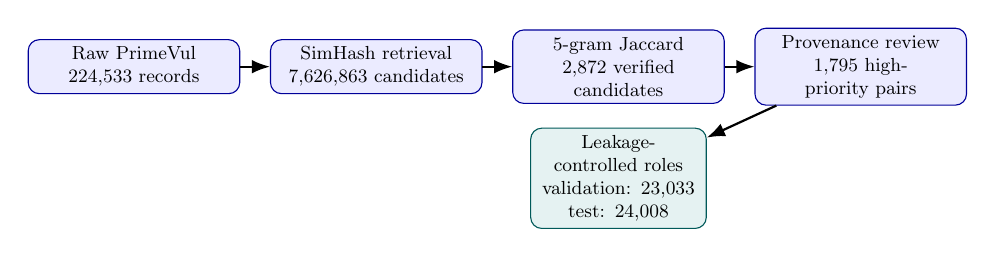
\begin{tikzpicture}[node distance=4mm and 5mm, scale=.76, transform shape]
  \node[paperbox] (raw) {Raw PrimeVul\\224,533 records};
  \node[paperbox, right=of raw] (sim) {SimHash retrieval\\7,626,863 candidates};
  \node[paperbox, right=of sim] (jac) {5-gram Jaccard\\2,872 verified candidates};
  \node[paperbox, right=of jac] (prov) {Provenance review\\1,795 high-priority pairs};
  \draw[paperarrow] (raw) -- (sim);
  \draw[paperarrow] (sim) -- (jac);
  \draw[paperarrow] (jac) -- (prov);
  \node[papersmall, below=of jac] (roles) {Leakage-controlled roles\\validation: 23,033\\test: 24,008};
  \draw[paperarrow] (prov) -- (roles);
\end{tikzpicture}
\caption{Leakage-control workflow used before model evaluation. Approximate lexical candidates were triaged and then reviewed for provenance; they were not automatically treated as confirmed semantic duplicates.}
\label{fig:leakage-flow}
\end{figure}

\subsection{LLM inference}

The model is \texttt{Qwen/Qwen2.5-Coder-1.5B-Instruct}, pinned to Hugging Face revision \texttt{2e1fd39}. The prompt contains the function code and requests a binary \texttt{YES}/\texttt{NO} verdict. CWE, CVE, project, commit, file, and hash metadata are retained for analysis but are not placed in the initial prompt. Greedy decoding, a fixed seed of 12345, FP16 inference, a maximum input length of 4,096 tokens, and a maximum output length of 16 tokens were used for reproducibility and practical GPU memory use.

The retained validation partition was processed first. It was used for calibration and policy selection. The retained test partition was processed only after the policy was frozen.

\subsection{Calibration and selective gate}

Temperature scaling was fitted on validation results. The fitted temperature was 445.683640902898 on the model's raw score scale. Platt scaling was also evaluated, but it did not produce a useful positive decision branch at the intended threshold. The primary conformal significance level was $\alpha=0.10$, selected under the validation protocol and frozen before the official test evaluation.

The selective decision was not ordinary binary classification. A record could be accepted as a positive alert or abstained. For the hybrid policy, the positive decision rule was:
\begin{equation}
\text{ACCEPT}=1 \quad \text{iff} \quad \mathcal{C}(x)=\{1\}\ \text{and Semgrep}(x)=1,
\label{eq:gate}
\end{equation}
where $\mathcal{C}(x)$ is the calibrated conformal prediction set. All remaining records were treated as abstentions for the selective policy.

\subsection{Static corroboration}

Semgrep Community Edition 1.163.0 was applied using the project C/C++ rule pack. The scanner processed the project-held-out candidate in batches of 512. A Semgrep finding was evidence of a matching rule, not proof of a vulnerability. No finding was treated as neutral rather than as evidence of safety.

\subsection{Evaluation metrics and uncertainty}

Accepted-positive precision is the proportion of accepted positive alerts that are truly vulnerable. Vulnerable-record recall is the proportion of all vulnerable records that are accepted as positive. Coverage is the proportion of all records receiving an accepted automatic decision. Because the system abstains, ordinary accuracy is not the primary metric.

Point estimates were supplemented with 5,000 record-level paired bootstrap resamples and 5,000 project-clustered resamples. Project clustering samples whole projects rather than individual functions because functions from the same project may be statistically related.

\section{Results}\label{sec:results}

\subsection{Raw baseline and locked-test comparison}

The official locked test contains 24,008 retained records, including 522 vulnerable records and 23,486 non-vulnerable records. Raw Qwen produced positive alerts for 23,788 records. The selective policies accepted substantially fewer records.

\begin{table}[htbp]
\caption{Official locked-test point estimates. Accepted-positive precision is calculated only among accepted positive alerts; abstentions are not counted as negative predictions.}\label{tab:locked}
\centering
{\small
\begin{tabular}{@{}lrrrrrrr@{}}
\toprule
Method & Alerts & TP & FP & Abstain & Coverage & Precision & Recall\\
\midrule
Raw Qwen & 23,788 & 479 & 23,309 & 220 & 99.08\% & 2.01\% & 91.76\%\\
Temp. + conformal & 2,319 & 108 & 2,211 & 21,689 & 9.66\% & 4.66\% & 20.69\%\\
Semgrep only & 1,514 & 104 & 1,410 & 22,494 & 6.31\% & 6.87\% & 19.92\%\\
Frozen hybrid & 452 & 36 & 416 & 23,556 & 1.88\% & 7.96\% & 6.90\%\\
\bottomrule
\end{tabular}}
\end{table}

\begin{figure}[htbp]
\centering
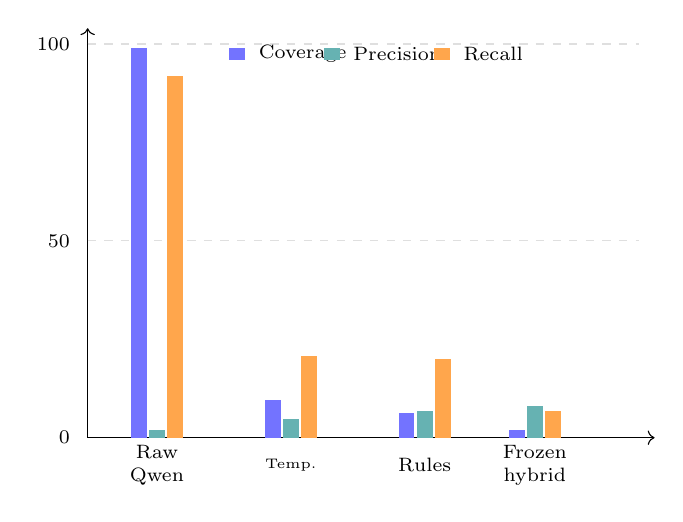
\begin{tikzpicture}
  \draw[->] (0,0) -- (7.2,0);
  \draw[->] (0,0) -- (0,5.2);
  \node[anchor=east,font=\scriptsize] at (-.1,5.0) {100};
  \node[anchor=east,font=\scriptsize] at (-.1,2.5) {50};
  \node[anchor=east,font=\scriptsize] at (-.1,0) {0};
  \draw[gray!25,dashed] (0,2.5) -- (7,2.5);
  \draw[gray!25,dashed] (0,5) -- (7,5);
  \fill[blue!55] (0.55,0) rectangle (0.75,4.954);
  \fill[teal!60] (0.78,0) rectangle (0.98,0.1005);
  \fill[orange!70] (1.01,0) rectangle (1.21,4.588);
  \fill[blue!55] (2.25,0) rectangle (2.45,0.483);
  \fill[teal!60] (2.48,0) rectangle (2.68,0.233);
  \fill[orange!70] (2.71,0) rectangle (2.91,1.0345);
  \fill[blue!55] (3.95,0) rectangle (4.15,0.3155);
  \fill[teal!60] (4.18,0) rectangle (4.38,0.3435);
  \fill[orange!70] (4.41,0) rectangle (4.61,0.996);
  \fill[blue!55] (5.35,0) rectangle (5.55,0.094);
  \fill[teal!60] (5.58,0) rectangle (5.78,0.398);
  \fill[orange!70] (5.81,0) rectangle (6.01,0.345);
  \node[font=\scriptsize, text width=1.3cm, align=center] at (0.88,-.35) {Raw Qwen};
  \node[font=\tiny, text width=.8cm, align=center] at (2.58,-.35) {Temp.};
  \node[font=\scriptsize, text width=1.0cm, align=center] at (4.28,-.35) {Rules};
  \node[font=\scriptsize, text width=1.4cm, align=center] at (5.68,-.35) {Frozen hybrid};
  \fill[blue!55] (1.8,4.8) rectangle (2.0,4.95); \node[anchor=west,font=\scriptsize] at (2.05,4.875) {Coverage};
  \fill[teal!60] (3.0,4.8) rectangle (3.2,4.95); \node[anchor=west,font=\scriptsize] at (3.25,4.875) {Precision};
  \fill[orange!70] (4.4,4.8) rectangle (4.6,4.95); \node[anchor=west,font=\scriptsize] at (4.65,4.875) {Recall};
\end{tikzpicture}
\caption{Official locked-test comparison. The frozen hybrid improves precision among accepted alerts, but the gain is accompanied by substantially lower coverage and vulnerable-record recall.}
\label{fig:locked-comparison}
\end{figure}

The frozen hybrid has the highest accepted-positive precision among the compared official-test policies. Its precision is 5.95 percentage points higher than raw Qwen, but its coverage and vulnerable-record recall are much lower. This is the expected cost of strict selective acceptance, not evidence that the hybrid is a complete vulnerability detector.

\subsection{Statistical uncertainty}

The precision advantage of the frozen hybrid over raw Qwen was +5.95 percentage points with a record-level 95\% interval of +3.60 to +8.54 and a project-clustered interval of +3.48 to +8.75. The precision advantage over temperature/conformal-only acceptance was +3.31 points under both resampling units. The difference from Semgrep-only precision included zero and is not reported as a statistically established improvement.

\begin{table}[htbp]
\caption{Frozen-hybrid paired differences on the official locked test. Values are percentage points.}\label{tab:paired}
\centering
{\small
\begin{tabular}{@{}lrrr@{}}
\toprule
Comparator & Coverage difference & Precision difference & Recall difference\\
\midrule
Raw Qwen & -97.20 & +5.95 & -84.87\\
Temp. + conformal & -7.78 & +3.31 & -13.79\\
Semgrep only & -4.42 & +1.10 & -13.03\\
\bottomrule
\end{tabular}}
\end{table}

\subsection{Project-held-out candidate}

The separate candidate contains 38,362 records from 400 projects absent from the official validation and test partitions, including 1,078 vulnerable records. It was used as an independent operating-point check and did not change the official locked-test result.

\begin{table}[htbp]
\caption{Project-held-out policy comparison.}\label{tab:holdout}
\centering
\begin{tabular}{@{}lrrrr@{}}
\toprule
Policy & Accepted & Abstain & Coverage & Precision / Recall\\
\midrule
Frozen $\alpha=0.10$ & 1,108 & 37,254 & 2.89\% & 11.01\% / 11.32\%\\
Higher-recall $\alpha=0.50$ & 3,071 & 35,291 & 8.01\% & 8.86\% / 25.23\%\\
\bottomrule
\end{tabular}
\end{table}

\begin{figure}[htbp]
\centering
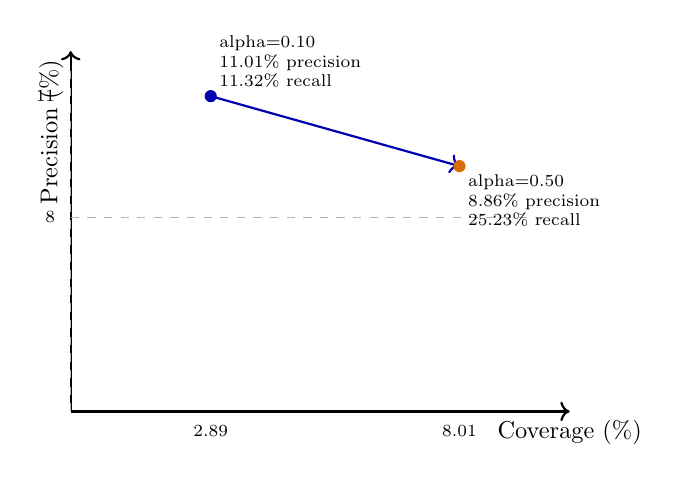
\begin{tikzpicture}[scale=.88, transform shape]
  \draw[->, thick] (0,0) -- (7.2,0) node[below] {Coverage (\%)};
  \draw[->, thick] (0,0) -- (0,5.2) node[left, rotate=90, yshift=8pt] {Precision (\%)};
  \draw[gray!60,dashed] (0,2.8) -- (7,2.8);
  \draw[gray!60,dashed] (0,0) -- (0,5);
  \node[anchor=east,font=\scriptsize] at (-.1,2.8) {8};
  \node[anchor=east,font=\scriptsize] at (-.1,4.55) {11};
  \node[anchor=north,font=\scriptsize] at (2.02,-.08) {2.89};
  \node[anchor=north,font=\scriptsize] at (5.61,-.08) {8.01};
  \draw[thick,blue!70!black,->] (2.02,4.55) -- (5.61,3.54);
  \fill[blue!70!black] (2.02,4.55) circle (2.5pt);
  \fill[orange!85!black] (5.61,3.54) circle (2.5pt);
  \node[anchor=south west, font=\scriptsize, text width=2.5cm] at (2.02,4.55) {alpha=0.10\\11.01\% precision\\11.32\% recall};
  \node[anchor=north west, font=\scriptsize, text width=2.7cm] at (5.61,3.54) {alpha=0.50\\8.86\% precision\\25.23\% recall};
\end{tikzpicture}
\caption{Project-held-out operating-point trade-off. A more permissive conformal level increases coverage and recall, but decreases accepted-alert precision.}
\label{fig:holdout-tradeoff}
\end{figure}

The alpha 0.50 candidate minus alpha 0.10 difference was +5.12 percentage points in coverage, -2.15 points in precision, and +13.91 points in recall. Project-clustered 95\% intervals were +4.13 to +6.19, -3.45 to -0.89, and +11.29 to +16.57 points, respectively. The candidate therefore demonstrates a stable precision--recall trade-off rather than an across-the-board improvement.

\subsection{Static corroboration}

On the project-held-out candidate, Semgrep found a static pattern in 3,654 of 38,362 records. Static positive precision was 8.95\% and static positive recall was 30.33\%. Qwen and Semgrep were classified as AGREE on 3,509 records, DISAGREE on 1 record, and NEUTRAL on 34,852 records. The large neutral group is expected because absence of a rule finding was not converted into a negative security claim.

\section{Discussion}\label{sec:discussion}

\subsection{What improved and what did not}

The principal improvement is precision among accepted alerts. Raw Qwen flags almost the entire official test set and has 2.01\% precision. The frozen hybrid accepts only 1.88\% of records and raises accepted-positive precision to 7.96\%. This is useful for a review-triage setting in which developers prefer a smaller number of stronger alerts.

The cost is substantial. Vulnerable-record recall falls from 91.76\% for raw Qwen to 6.90\% for the frozen hybrid because most records are abstained or fail the corroboration gate. The system therefore cannot be described as a high-recall autonomous detector. It is a conservative alert-prioritization mode.

\subsection{Role of the components}

Temperature/conformal-only acceptance and Semgrep-only acceptance retain more vulnerable records than the intersection hybrid, while the hybrid has the highest accepted precision. This indicates that the strict intersection of calibrated confidence and rule evidence is the main source of conservatism. The result supports reporting component ablations rather than presenting only the final pipeline score.

\subsection{Interpretation of the project-held-out result}

The project-held-out candidate provides a useful generalization check for the selected policies because its projects were absent from official validation and test. The higher-recall alpha 0.50 setting accepts more records and more vulnerable records, but also more false positives. Because the candidate is a separate derived evaluation population rather than the original benchmark test, it should be reported as an auxiliary project-held-out study and not substituted for the locked-test result.

\subsection{Practical value}

The pipeline is most appropriate when automated review is used to prioritize human attention. It can produce a high-precision queue of cases with two types of supporting evidence and route the remaining cases for manual inspection. The design makes the cost of caution visible through coverage and abstention rate instead of hiding it in a single accuracy value.

\section{Threats to Validity and Limitations}\label{sec:limitations}

\textbf{Construct validity.} PrimeVul labels provide a useful binary benchmark, but real code review includes severity, vulnerability type, exploitability, and repairability. A binary target cannot represent all of that nuance.

\textbf{Internal validity.} Calibration and policy choices were made using validation data, and the official test was locked. Nevertheless, the leakage audit is conservative: approximate similarity and provenance evidence identify records requiring review but do not establish semantic duplication for every pair.

\textbf{Model scope.} The completed study evaluates one primary open-source model, Qwen2.5-Coder-1.5B-Instruct. The results do not establish universal superiority over other LLMs.

\textbf{Static-analysis scope.} Semgrep was applied with a function-local rule pack. The absence of a finding is neutral, and the rule pack is not equivalent to repository-level CodeQL or industrial SAST deployment.

\textbf{Metric scope.} The primary metrics are coverage, accepted-positive precision, and vulnerable-record recall. Reliability diagrams, AUROC, subgroup analyses, Pearson correlation, Cohen's kappa, verbal-confidence experiments, self-consistency, and ensemble calibration were not completed and are not presented as results.

\textbf{External validity.} The benchmark distribution and function-level context may differ from industrial repositories. The project-held-out candidate improves the evidence for project separation but does not establish universal unseen-project generalization.

\section{Conclusion}\label{sec:conclusion}

This study evaluated a confidence-calibrated and selective LLM pipeline for automated code-review triage. A raw Qwen baseline was combined with validation-only temperature calibration, conformal-style abstention, and Semgrep rule corroboration. The frozen hybrid increased accepted-alert precision from 2.01\% to 7.96\% on the official leakage-controlled test, with a large reduction in coverage and recall. A separate project-held-out candidate showed that a more permissive operating point can recover more vulnerable records, but precision decreases.

The findings support a cautious conclusion. Calibration, abstention, and corroboration can improve the quality of a small set of automatically accepted alerts, but they do not remove the need for human review and do not improve precision, recall, and coverage simultaneously. The resulting contribution is a reproducible reliability-aware triage framework with explicit operating-point trade-offs.

\backmatter

\bmhead{Data availability}
The raw PrimeVul files are retained in the project dataset directory. The raw JSONL partitions were not modified. The derived leakage-controlled manifest and project-held-out manifest record the evaluation roles and exclusions.

\bmhead{Code availability}
The inference, audit, calibration, Semgrep, policy, and statistical scripts are archived in the Thesis context package. The full absolute-path inventory is provided in the supervisor briefing document.

\bmhead{Funding}
Not applicable.

\bmhead{Competing interests}
The author declares no competing interests.

\bmhead{Ethics approval}
Not applicable. The study uses public software-code benchmark records and does not involve human participants or human subjects.

\bmhead{Author contribution}
The author designed the study, implemented the analysis, evaluated the results, and prepared the manuscript.

\begin{appendices}
\section{Reproducibility configuration}\label{app:config}

\begin{table}[htbp]
\caption{Key configuration values used in the completed experiments.}\label{tab:config}
\centering
\begin{tabular}{@{}ll@{}}
\toprule
Component & Configuration\\
\midrule
Model & Qwen/Qwen2.5-Coder-1.5B-Instruct, revision 2e1fd39\\
Prompt & Code-only, binary YES/NO verdict\\
Seed & 12345\\
Input limit & 4,096 tokens\\
Output limit & 16 tokens\\
Calibration & Temperature scaling on retained validation\\
Primary alpha & 0.10\\
Static tool & Semgrep Community Edition 1.163.0\\
Hybrid gate & Conformal set exactly [1] and at least one Semgrep finding\\
Bootstrap & 5,000 record-level and 5,000 project-level resamples\\
\bottomrule
\end{tabular}
\end{table}

\section{Scopus search string}\label{app:search}

The main Scopus query used to identify the literature corpus was:

\begin{quote}\small
\texttt{TITLE-ABS-KEY: (large language model OR LLM) AND (software vulnerability OR automated code review) AND (calibration OR uncertainty OR abstention OR conformal prediction OR static analysis)}
\end{quote}

The export contained 77 Scopus records. The complete CSV and BibTeX exports
are retained with the manuscript artifacts.
\end{appendices}

\bibliography{paper_references}

\end{document}

